\documentclass{beamer}

\usepackage[T2A]{fontenc}
\usepackage[utf8]{inputenc}
\usepackage[russian, english]{babel}
%\usepackage{times}
\usepackage[labelfont=bf]{caption}
\usepackage[font=small,labelfont=bf]{subcaption}
\usetheme{Madrid}

%% For figures numbered by section
\usepackage{chngcntr}
\counterwithin{figure}{section}
\counterwithin{table}{section}

%% For bookmarks
\usepackage{bookmark} 

%% Bibliography
\usepackage[backend=bibtex,
natbib=true, 
style=chicago-authordate]{biblatex}
\addbibresource{Returns.bib}
\def\bibfont{\small}

%% For color in text
\usepackage{xcolor}

%% For sparklines in table
\usepackage{graphicx} 
\usepackage{lmodern} 
\newcommand{\graph}[3]{
	\raisebox{-#1mm}{\includegraphics[height=#2em,width=2cm]{#3}}
}

%% For tables in panel
\usepackage{ltablex,ragged2e}
\renewcommand\tabularxcolumn[1]{>{\RaggedLeft}p{#1}}

%% For own made graphs
\usepackage{tikz}

\usepackage{relsize}
\usepackage{tabularx}
\usepackage{tabulary}
\usepackage{multirow}

\title[]{Может ли обесценение человеческого капитала объяснить тенденции в отдаче от образования в Российской Федерации?}
\author{Сухас Д. Парандекар}
\date[Семинар Всемирного банка, 2020]{Отдача от образования в Российской Федерации, 2020}

\begin{document}
	
%%%%%%%%%%	
\begin{frame}
	\titlepage
\end{frame}

%%%%%%%%%%	
\begin{frame}{Содержание презентации}
	\tableofcontents
\end{frame}
	
%%%%%%%%%%
\section{Мотивация}

\subsection{Текущая ситуация в области человеческого капитала в России}
\subsection{Временной тренд в отдаче от образования}

%%%%%%%%%%
\begin{frame}{Мотивация}{Темпы отдачи от человеческого капитала в целом и в зависимости от пола}
	\centering
	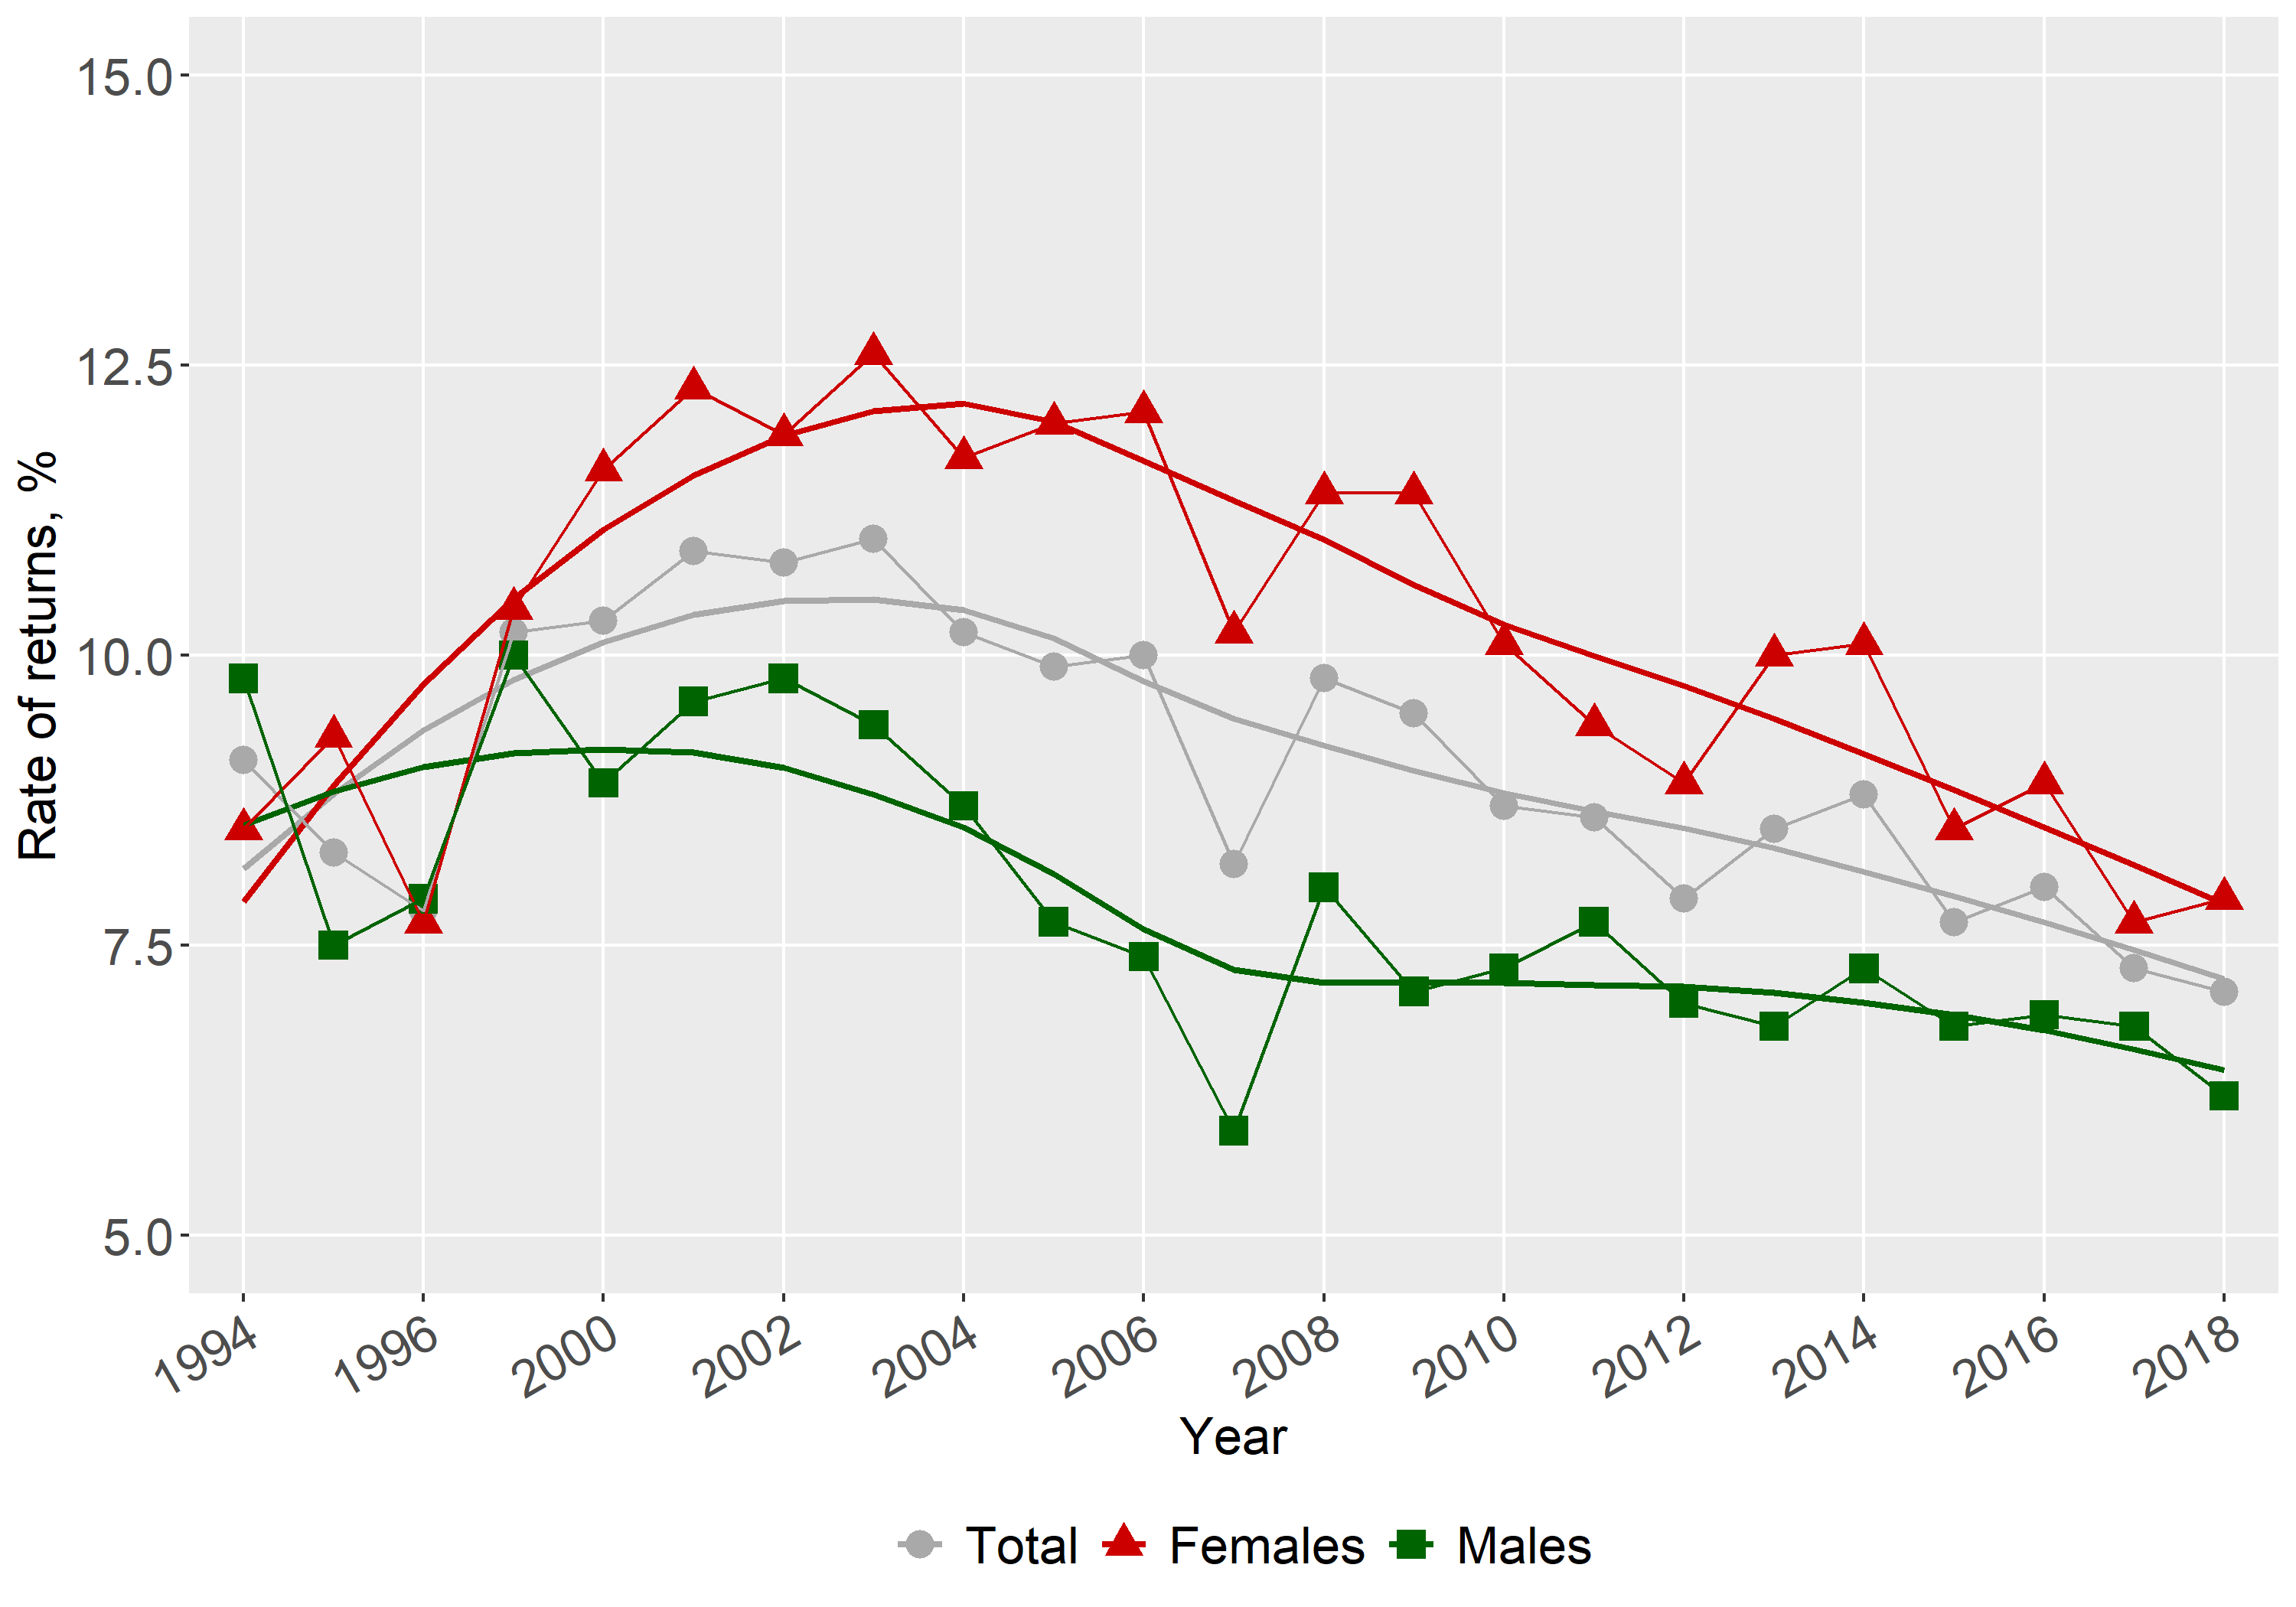
\includegraphics[width=260pt, height=200pt]{re_edu.png}
\end{frame}

%%%%%%%%%%
\begin{frame}{Результаты анализа отдачи от человеческого капитала}{Совместное изменение во времени уровней отдачи от профессионального и высшего образования в разбивке по полу  в России}
	\begin{figure}
		\centering
		\subfloat[Женщины]{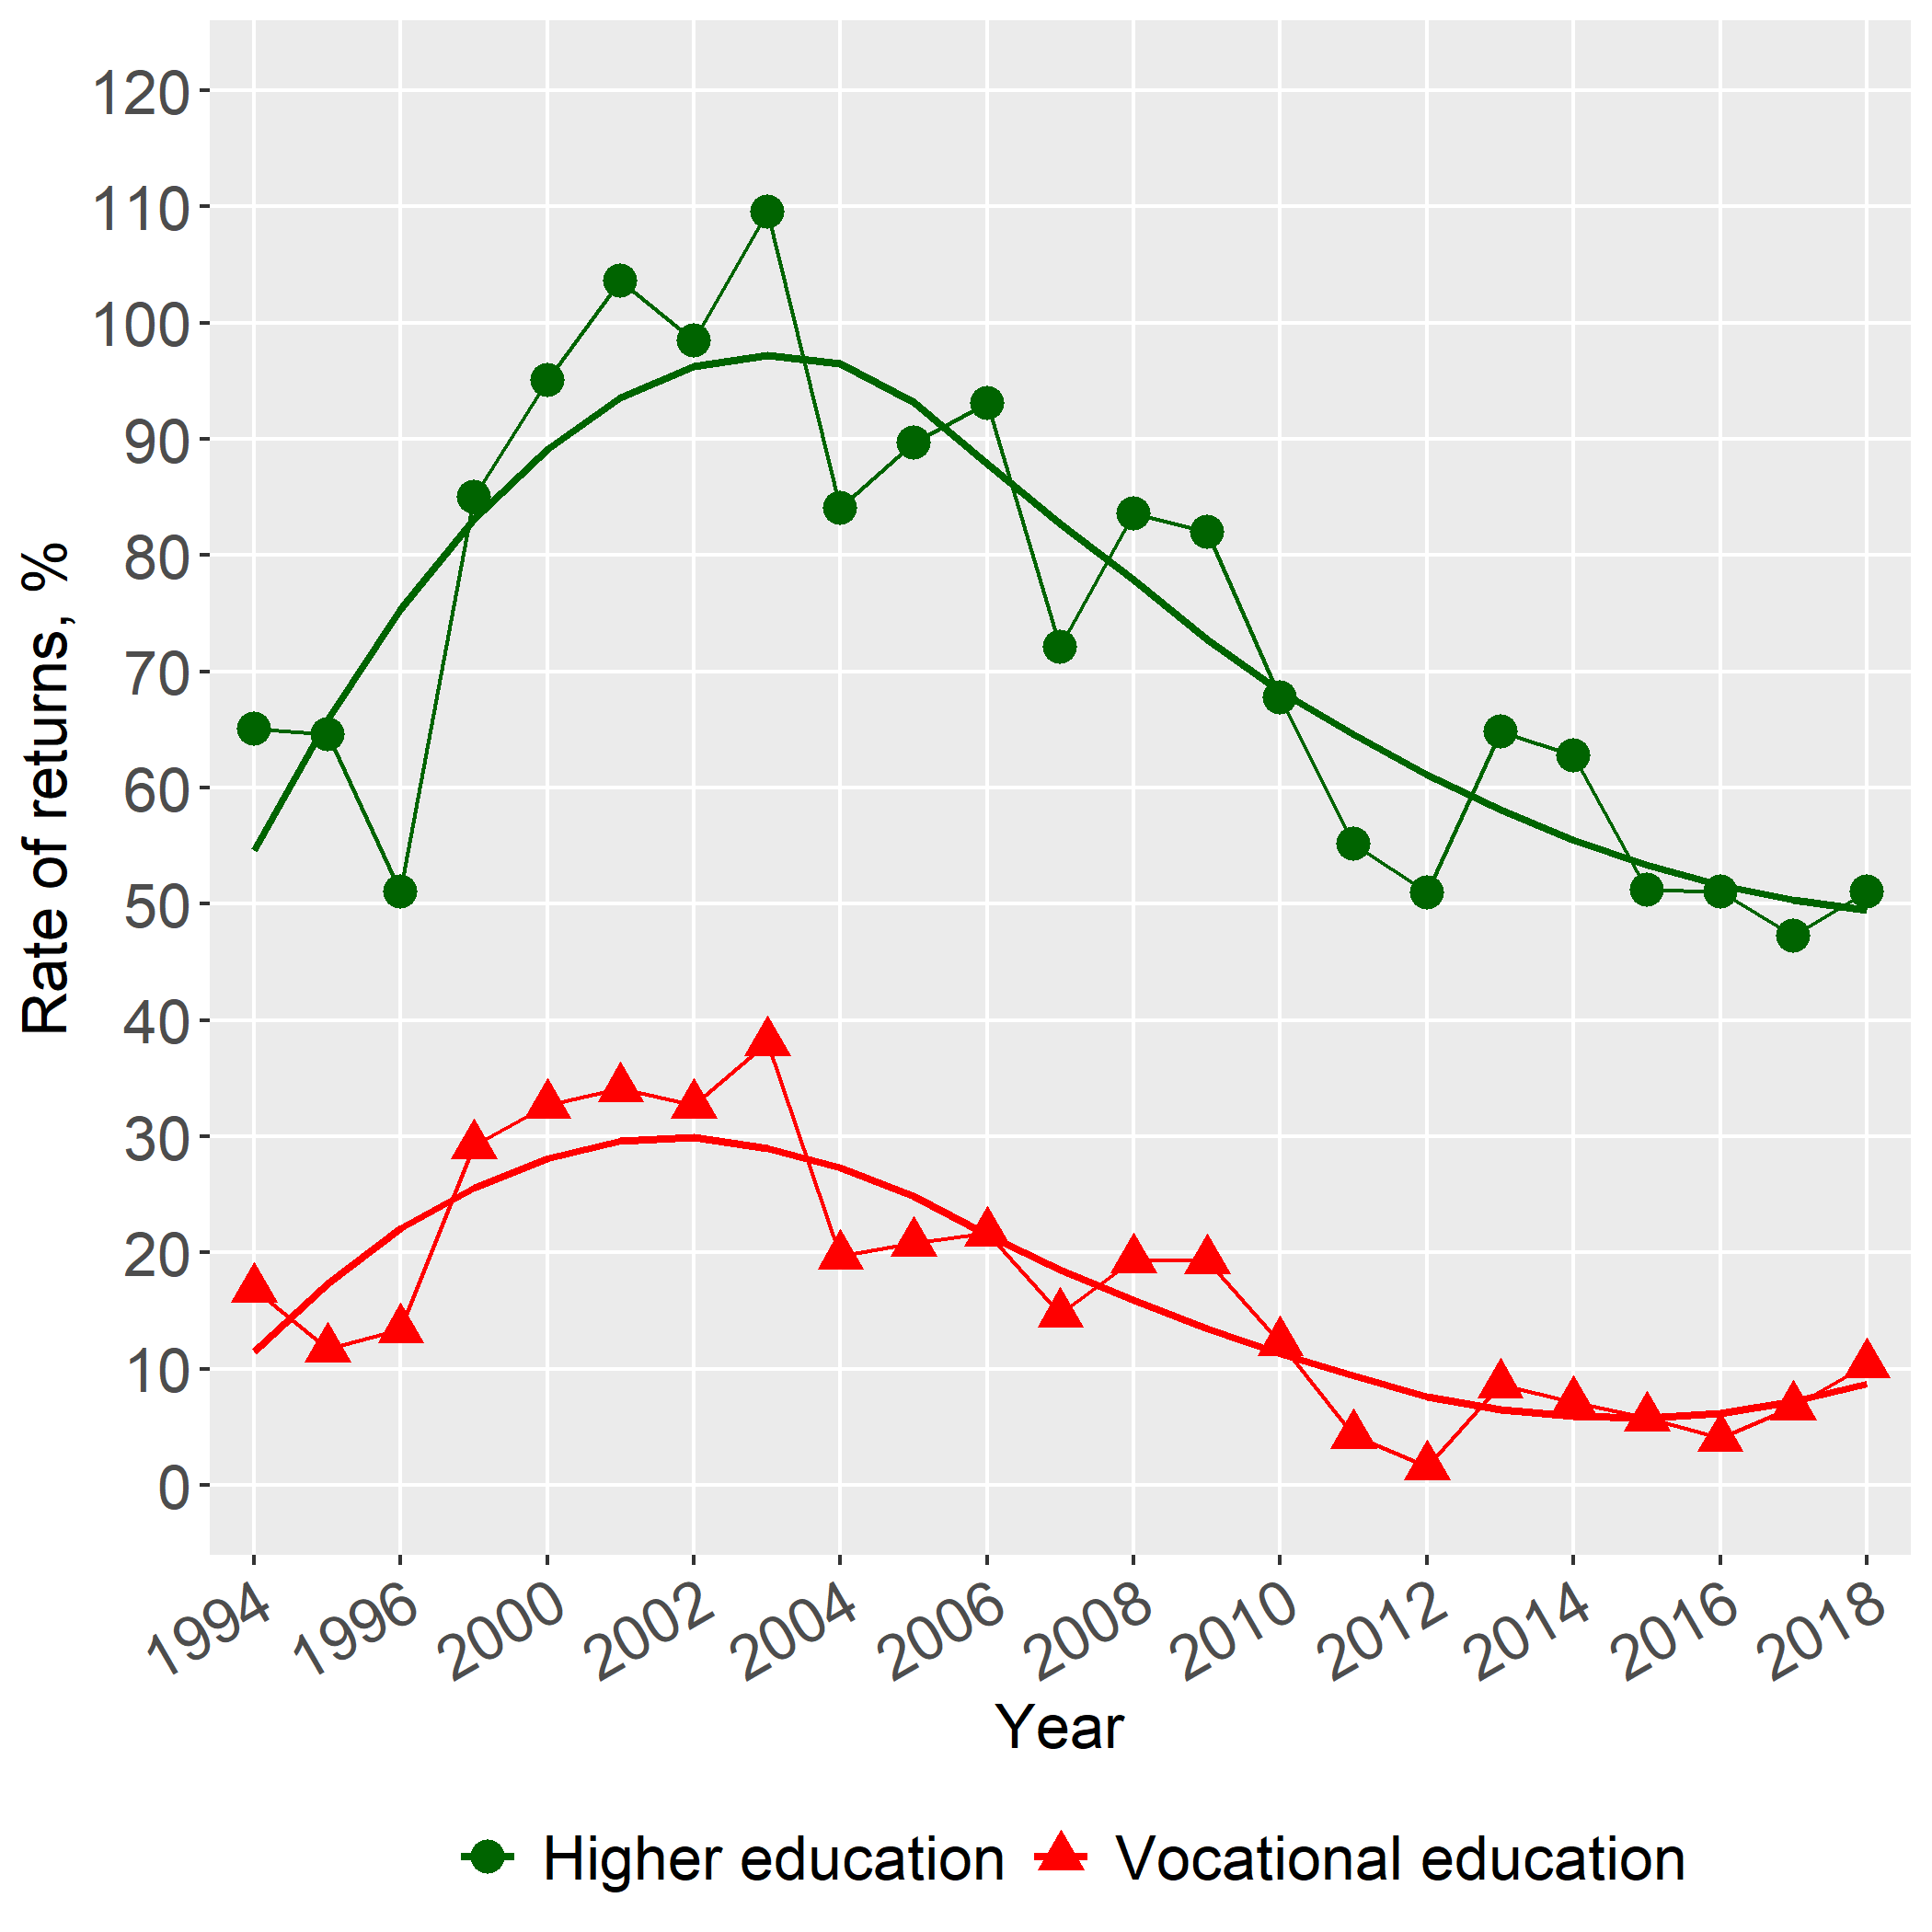
\includegraphics[width=150pt]{re_HE_f.png}}
		\hfill
		\subfloat[Мужчины]{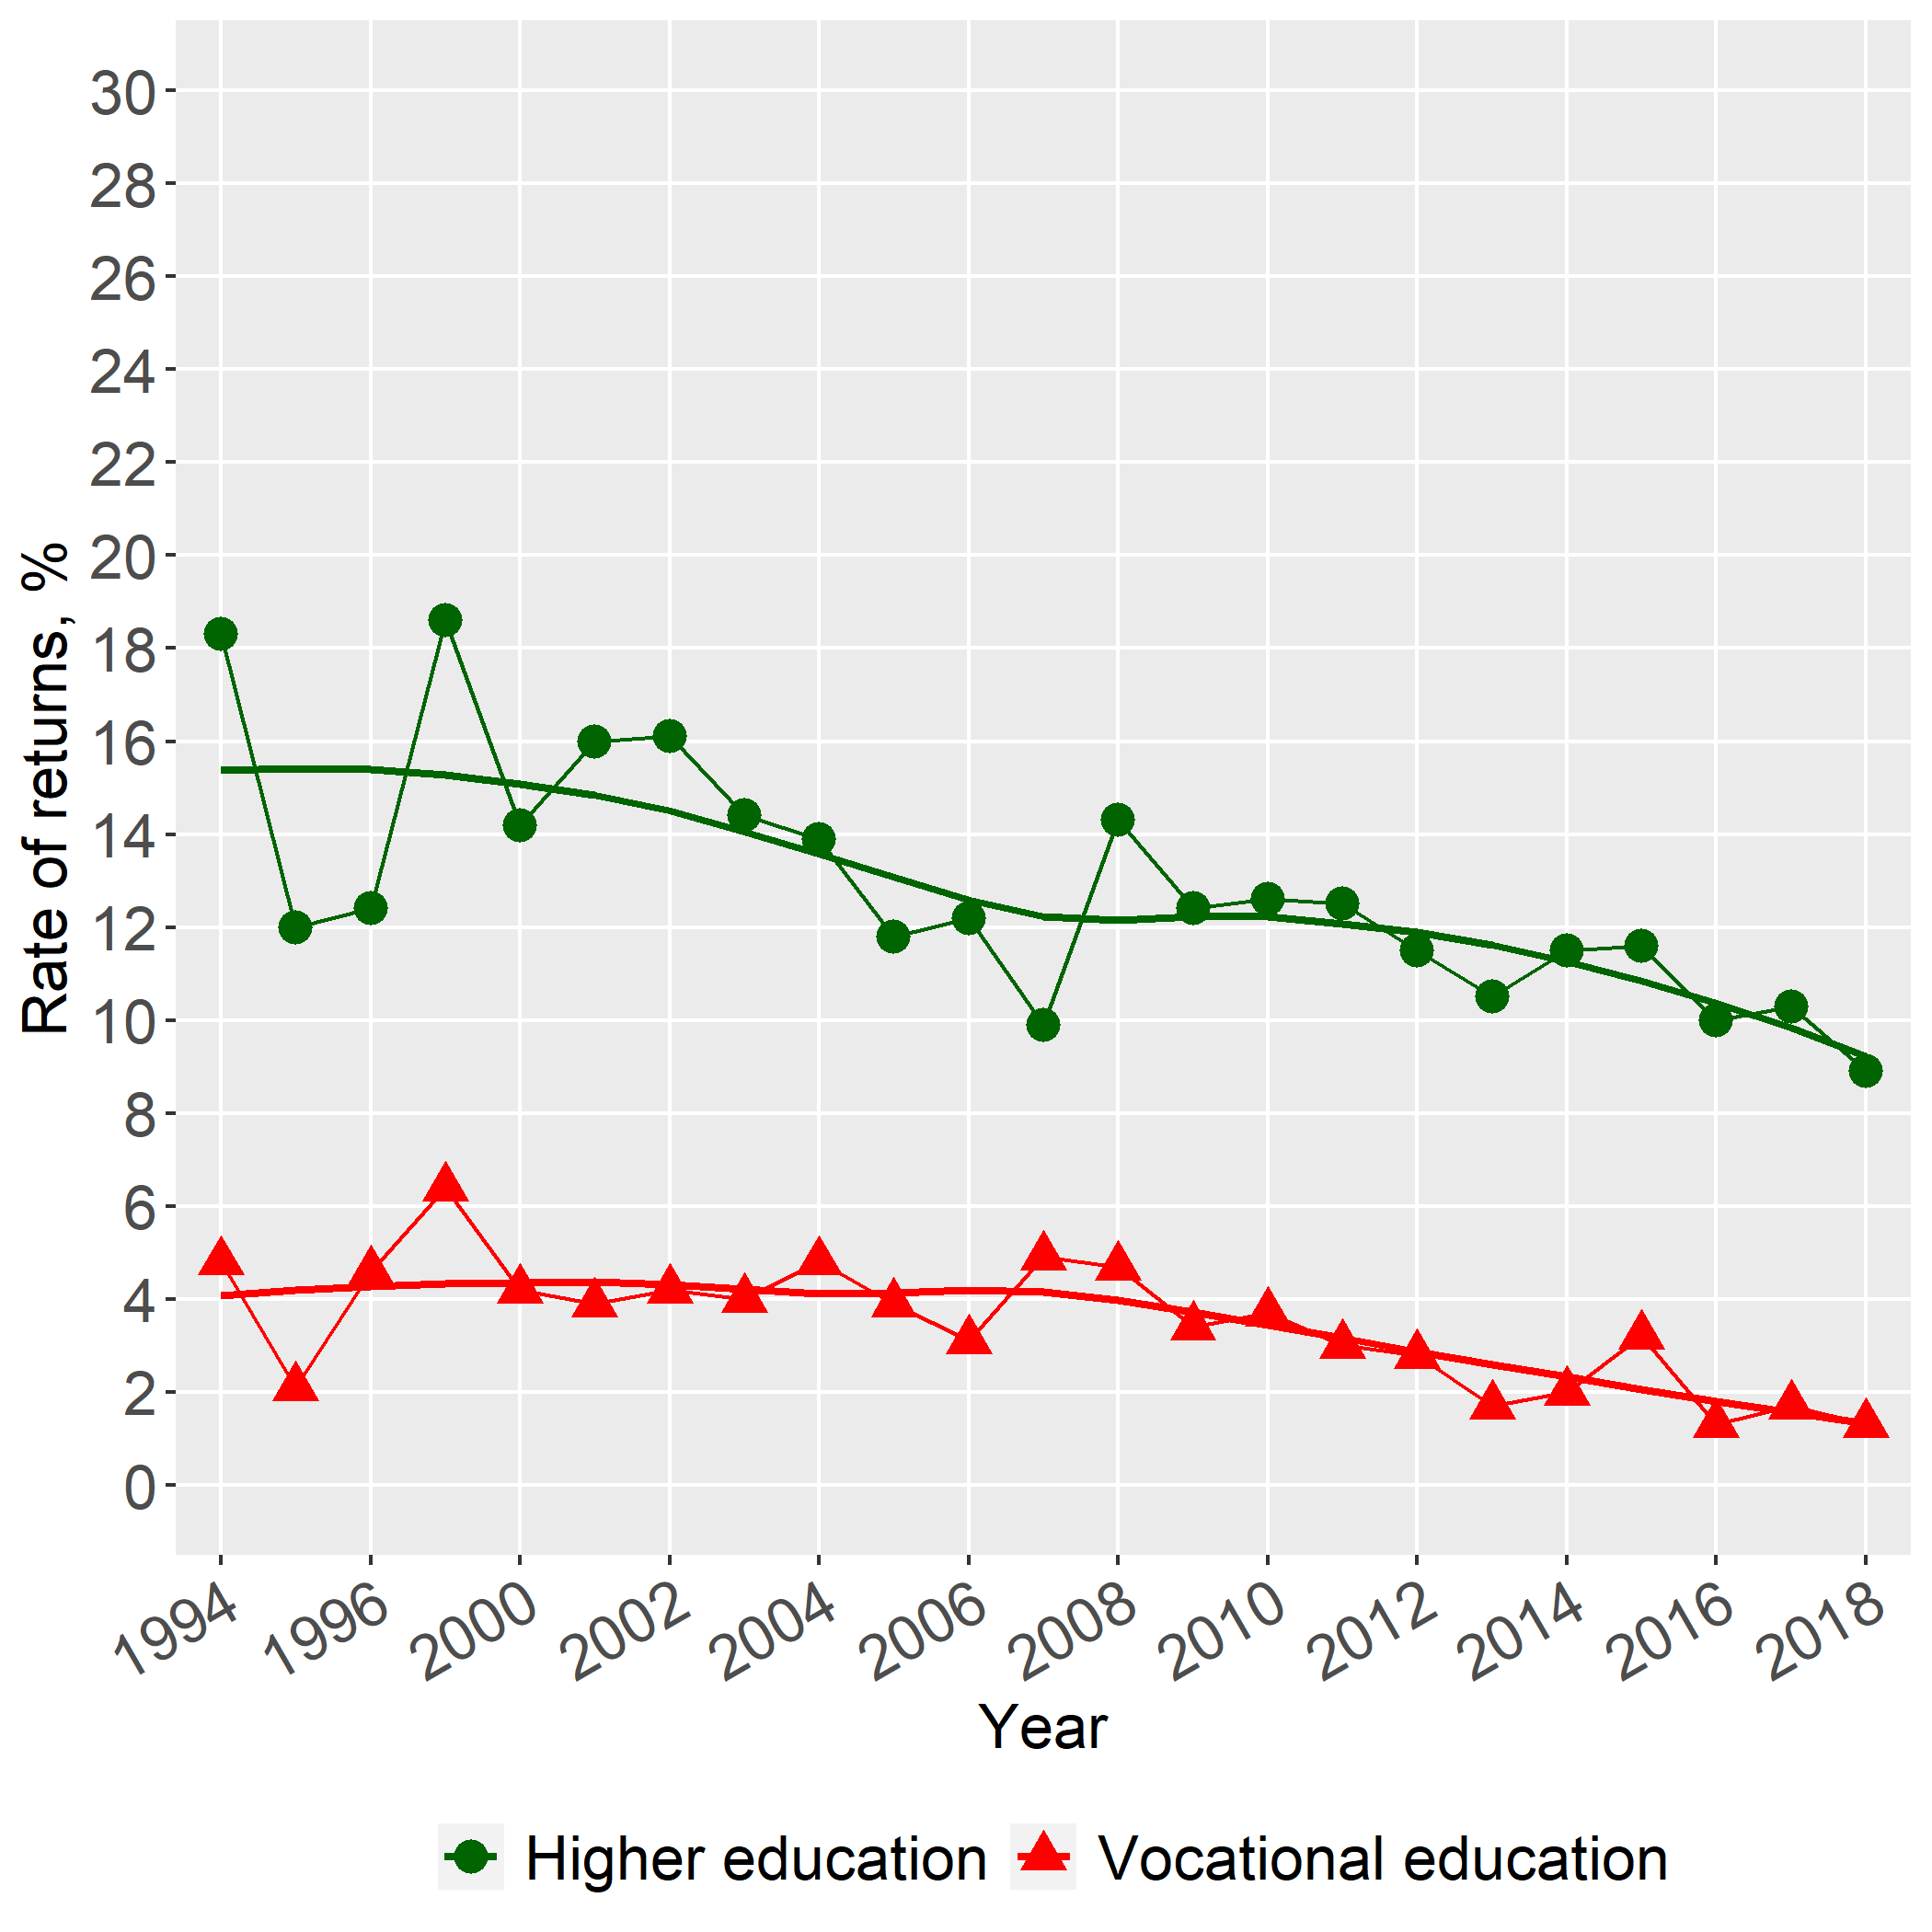
\includegraphics[width=150pt]{re_HE_m.png}}
	\end{figure}
\fontsize{8}{10}\selectfont
	\begin{itemize}
		\vspace*{-0.2in}
		\item Для мужчин отдача от образования почти не меняется со временем.
		\item Для женщин отдача от образования растет до начала нулевых, а затем снижается.
	\end{itemize}
\end{frame}



%%%%%%%%%%
\begin{frame}{Мотивация}{Пик поступления в высшие учебные заведения (Ежегодник НИУ ВШЭ)}
\begin{figure}
	\centering
	\vspace*{-0.2in}
	\hspace*{-0.3in}
	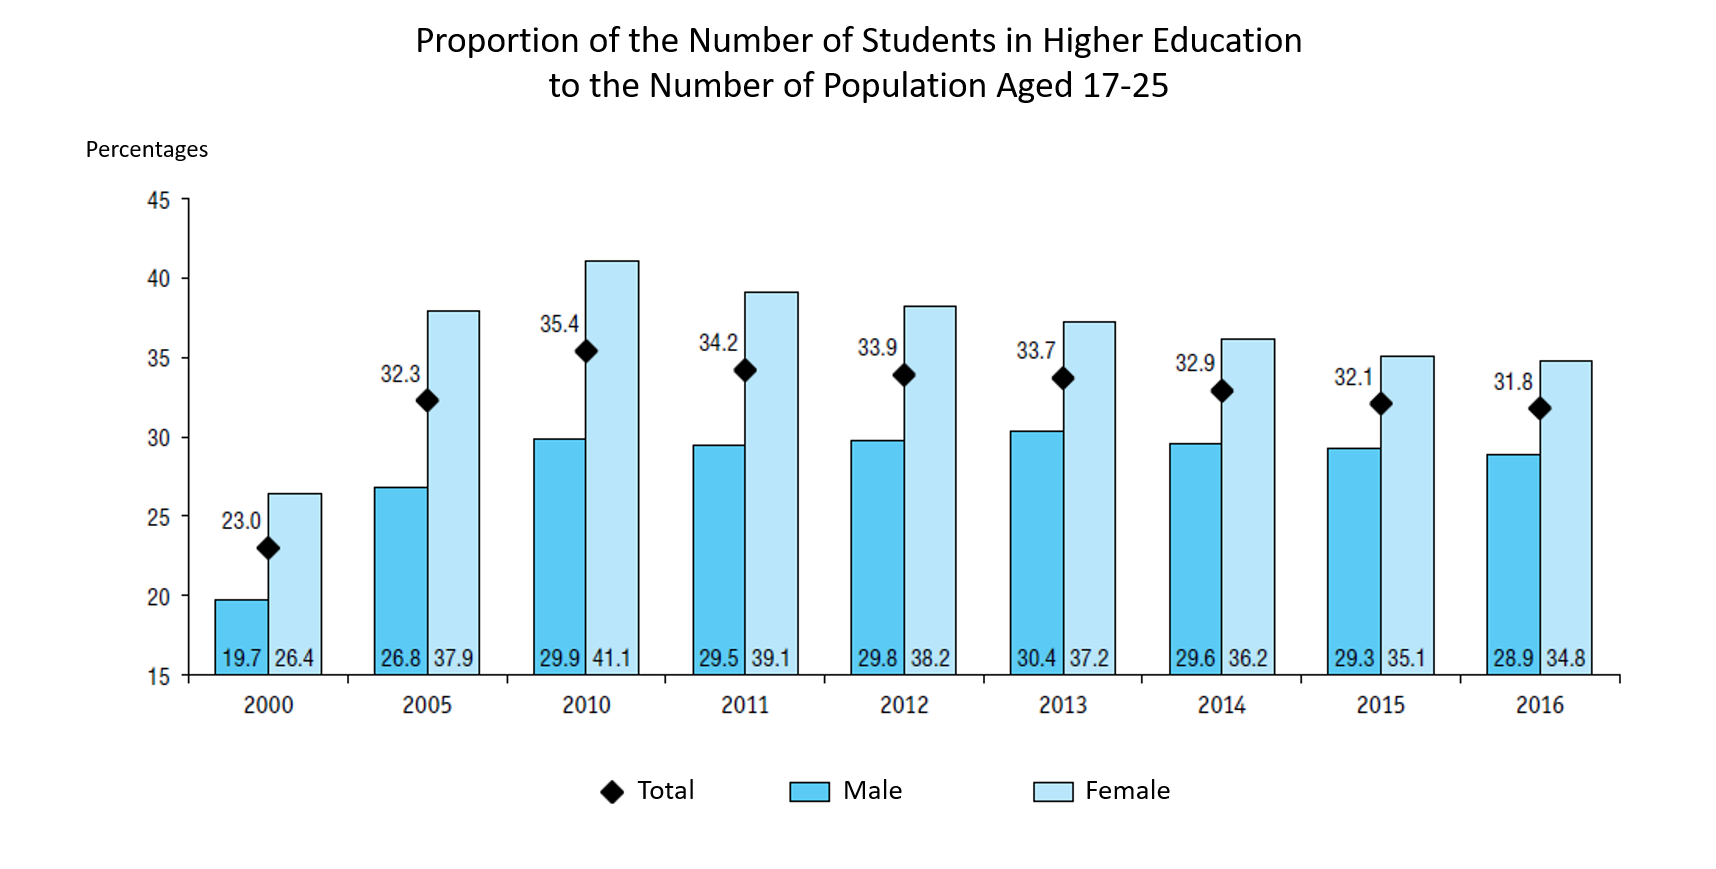
\includegraphics[width=350pt, height=200pt]{graph_1b.png}
\end{figure}
\end{frame}
	

%%%%%%%%%%
\section{Обесценение человеческого капитала в России}
\subsection{Аналитический подход к изучению обесценения}

%%%%%%%%%%
\begin{frame}{Обесценение человеческого капитала в России}{"Винтажные эффекты" Неймана-Вайса по уровням образования}
\begin{figure}
	\centering
	\subfloat[Высшее]{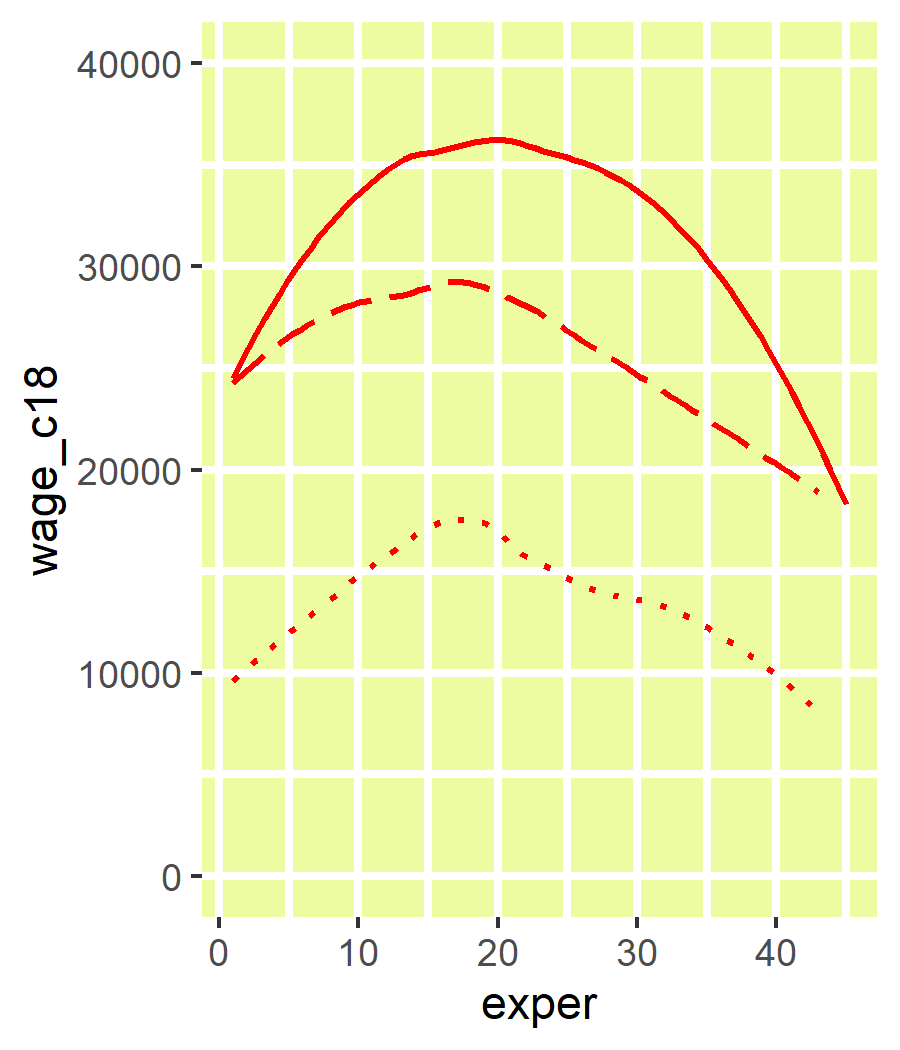
\includegraphics[width=110pt]{dp01_he.png}}
	\hfill
	\subfloat[Профессиональное]{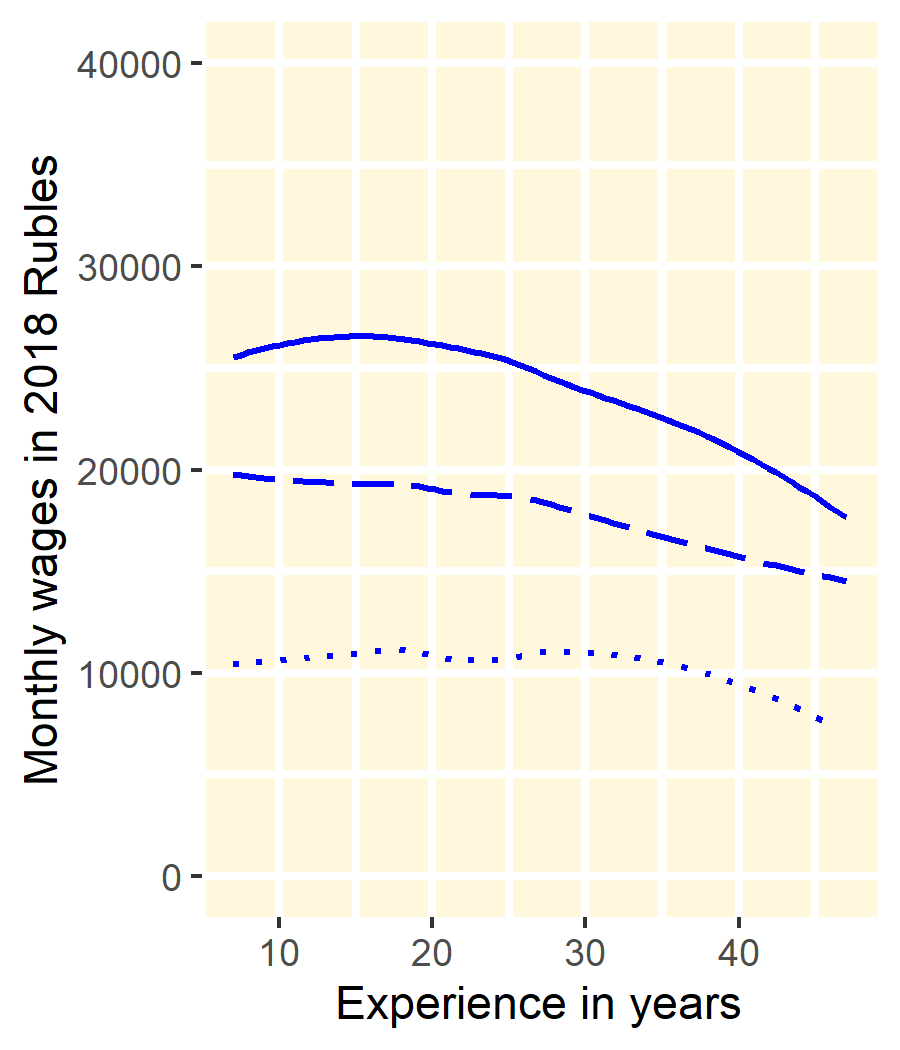
\includegraphics[width=110pt]{dp01_ve.png}}
	\hfill
	\subfloat[Среднее]{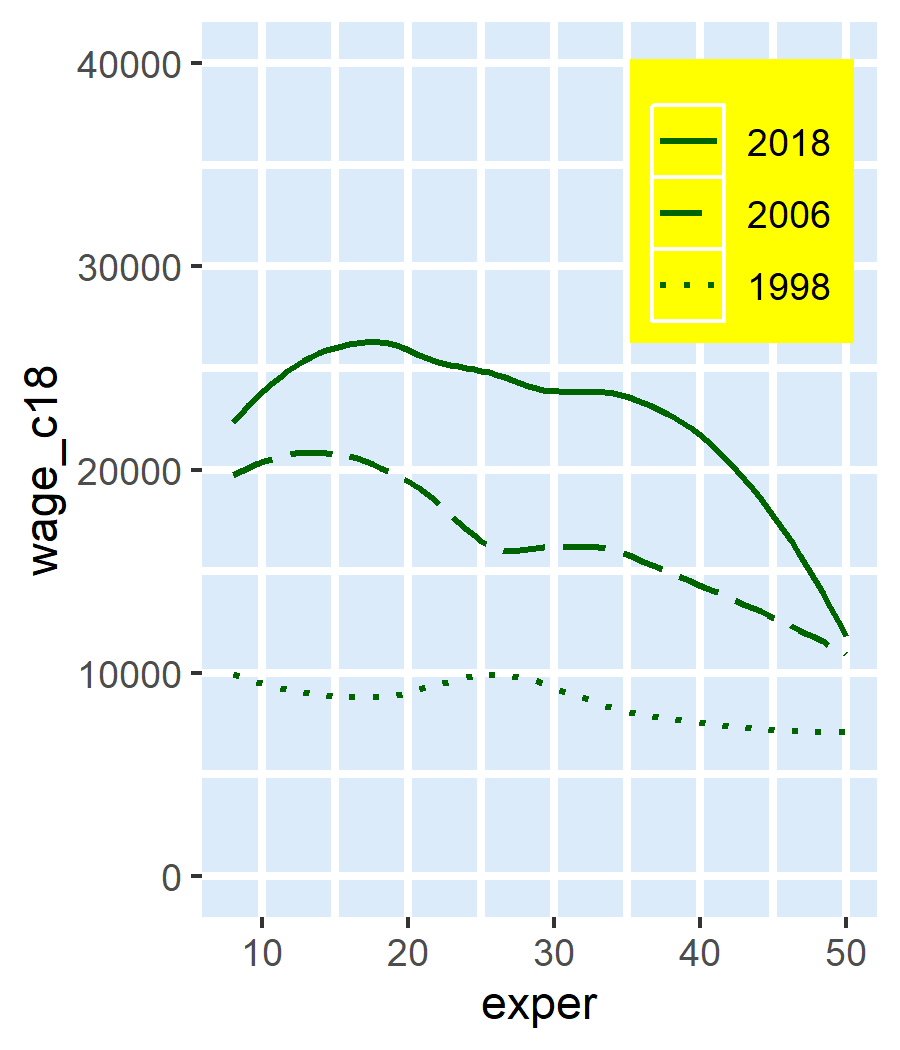
\includegraphics[width=110pt]{dp01_se.png}}
\end{figure}
\fontsize{8}{10}\selectfont
\begin{itemize}
	\item Вогнутый профиль характерен только для высшего образования. 
	\item Для профессионального и среднего образования вогнутый профиль менее выражен.
	\item Необходим более строгий аналитический подход к изучению данного вопроса.
\end{itemize}
\end{frame}

\begin{frame}{Обесценение человеческого капитала в России}{Аналитический подход в изучении обесценения}
	Два типа обесценения (потеря производственного потенциала человеческого капитала) \citep{neuman_091._1995}:
	\begin{itemize}
		\item \textbf{Внешнее обесценение} ("износ" или "винтажный эффект"): возникает вследствие общего обновления технологий или действия других рыночных сил, которые снижают ценность образования или профессиональной подготовки, полученных в предыдущий период.
		\item \textbf{Внутреннее обесценение}: возникает вследствие естественного ухудшения физических и умственных способностей человека с возрастом.
	\end{itemize}
\end{frame}

%%%%%%%%%%
\begin{frame}{Обесценение человеческого капитала в России}{Метод Мурильо}
\begin{itemize}
	\item Мурильо (2006) реализовал вариацию модели Неймана и Вайса (1995) с фокусом на эмпирическом применении к Испании.
	\item В целом модель может быть выражена следующим образом:
	
	\begin{equation}
	log(W) = \alpha +  \beta_{1}S + \pi_{1}TS + \beta_{2}T + \pi_{2}T^{2} 
	\end{equation}
	где $T$ -- трудовой стаж/опыт (лет), $S$ -- образование (лет), $\alpha$, $\beta_{1}$, $\beta_{1}$, $\pi_{1}$, $\pi_{2}$ -- регрессионные коэффициенты.
	\vspace{2pt}
	\item Уровень обесценения человеческого капитала в течение $T$ лет за счет образования может быть рассчитан как $\pi_{1}S $, а за счет опыта -- $ 2\pi_{2}T$.
\end{itemize}
\end{frame}

%%%%%%%%%%
\subsection{Результаты анализа}
\begin{frame}{Обесценение человеческого капитала в России}{Первоначальные результаты расчета уровня обесценения  человеческого капитала по годам}
	\fontsize{7}{10}\selectfont
	\begin{tabularx}{\textwidth}{rlrrrrrrc}
		\hline
		& \textbf{Показатель} & \textbf{1994} & \textbf{1998} & \textbf{2003} & \textbf{2006} & \textbf{2012} & \textbf{2018} &  \\ 
		\hline
		1 & \begin{tabular}[l]{@{}l@{}} Опыт (лет), \\ среднее \end{tabular}   & 21.41 & 22.32 & 22.20 & 22.24 & 22.52 & 22.52 & \\
		2 & \begin{tabular}[l]{@{}l@{}} Образование (лет), \\ среднее \end{tabular} & 12.70 & 12.69 & 12.79 & 12.79 & 12.95 & 13.27 &\\
		\hline
		3 & \begin{tabular}[l]{@{}l@{}} Обесценение \\ опыта, \% \end{tabular} & 1.87 & 1.55 & 1.04 & 0.50 & 1.37 & 1.63 & 
		\graph{1}{1}{C:/Country/Russia/Data/SEASHELL/SEABYTE/Edreru/wp1/sparklines/all2-1} \\ 
		4 & \begin{tabular}[l]{@{}l@{}} Обесценение \\ образования, \% \end{tabular} & 2.80 & 2.71 & 0.11 & 0.00 & 0.00 & 0.00 &
		\graph{1}{1}{C:/Country/Russia/Data/SEASHELL/SEABYTE/Edreru/wp1/sparklines/all2-2} \\ 
		5 & \begin{tabular}[l]{@{}l@{}} Обесценение \\ человеческого \\ капитала, \% \end{tabular}  & 4.67 & 4.26 & 1.15 & 0.50 & 1.37 & 1.63 & 
		\graph{1}{1}{C:/Country/Russia/Data/SEASHELL/SEABYTE/Edreru/wp1/sparklines/all2-3}\\ 
		\hline
	\end{tabularx}

\end{frame}

%%%%%%%%%%
\subsection{Нелинейный метод наименьших квадратов Арразолы}
	\subsection{Результаты анализа}
%%%%%%%%%%
\begin{frame}{Обесценение человеческого капитала в России}{Оценки нелинейного метода наименьших квадратов}
	\fontsize{9}{10}\selectfont
	\begin{itemize}
		\item Арразола и др. (2005) разработали альтернативный (нелинейный) подход к изучению обесценения человеческого капитала.
	\end{itemize}
		\fontsize{5}{6}\selectfont
		\keepXColumns
		\begin{tabularx}{\textwidth}{clccccccc}
			\hline
			& \textbf{Параметр} & \textbf{1994} & \textbf{1998} & \textbf{2003} & \textbf{2006} & \textbf{2012} & \textbf{2018} & \\ 
			\hline
			& \textbf{\begin{tabular}[l]{@{}l@{}} Обесценение \\ человеческого \\ капитала: \\ вся выборка \end{tabular}} & 0.0246 & 0.0208 & 0.0093 & -0.0040 & 0.0369 & 0.0459 & 
			\graph{1}{1}{C:/Country/Russia/Data/SEASHELL/SEABYTE/Edreru/wp1/sparklines/Weber_sprk_all2-1}\\ 
			
			&  & (0.0052) & (0.0043) & (0.0050) & (0.0058) & (0.0043) & (0.0051) & \\ 
			\hline
			
			& \textbf{\begin{tabular}[l]{@{}l@{}} Обесценение \\ человеческого \\ капитала: \\ женщины \end{tabular}} & 0.0275 & 0.0260 & 0.0156 & 0.0065 & 0.0197 & 0.0249 & 
			\graph{1}{1}{C:/Country/Russia/Data/SEASHELL/SEABYTE/Edreru/wp1/sparklines/Weber_sprk_f2-1}\\ 
			&  & (0.0060) & (0.0042) & (0.0038) & (0.0044) & (0.0036) & (0.0036) & \\ 
			\hline
			
			& \textbf{\begin{tabular}[l]{@{}l@{}} Обесценение \\ человеческого \\ капитала: \\ мужчины \end{tabular}} & 0.0261 & 0.0168 & -0.0020 & 0.0015 & 0.0595 & 0.0511 & 
			\graph{1}{1}{C:/Country/Russia/Data/SEASHELL/SEABYTE/Edreru/wp1/sparklines/Weber_sprk_m2-1}\\ 
			&  & (0.0067) & (0.0059) & (0.0082) & (0.0095) & (0.0063) & (0.0069) & \\
			\hline
			
		\end{tabularx}
	\fontsize{8}{10}\selectfont
\begin{itemize}
	\item Графики указывают на U-образный паттерн для обесценения (аналогично оценкам Мурильо): уровень износа человеческого капитала сначала уменьшается, а затем снова увеличивается. 
	\item Это подтверждает тезис о том, что наблюдаемый во времени рост, а затем снижение отдачи от образования в России можно объяснить эффектом обесценения.
\end{itemize}
\end{frame}		

%%%%%%%%%%
\section{Дальнейшее изучение обесценения}
	\subsection{Обесценение и гендерный аспект}

%%%%%%%%%%
\begin{frame}{Дальнейшее изучение обесценения}{Обесценение и гендерный аспект}
	\fontsize{8}{10}\selectfont
	\begin{itemize}
		\item Модель Неймана и Вайса дает оценку нормы обесценения человеческого капитала, но не позволяет определить, какая часть этой нормы является \textit{внешней}, а какая \textit{внутренней}.
		
		\item Исследование различий в норме обесценения с помощью \textbf{сегрегационной классификации} помогает решить данную проблему на основе следующей гипотезы.
		
		\item Предполагается, что \textit{внешнее обесценение} будет иметь большее влияние на \textbf{отрасль}, поскольку технологические изменения будут распространяться быстрее через отрасль, а не через \textbf{профессии}, которые рассеяны по отраслям.
		
		\item Причина этого в том, что профессии связаны с образованием, а изменения в образовании распространяются медленнее. Отрасли включают разнородные образовательные группы, в то время как профессии более однородны, и, следовательно, рыночные изменения влияют на отрасли быстрее.
	\end{itemize}
\end{frame}	
	
%%%%%%%%%%
\begin{frame}{Дальнейшее изучение обесценения}{Средние уровни обесценения человеческого капитала по "мужским" и "женским" отраслям и профессиям, РМЭЗ 2018}
		\fontsize{7}{9}\selectfont
		\centering 
		\label{tab:3.3} 
		\begin{tabularx}{\textwidth}{cl|cc|cc}
			\hline
			& \textbf{Показатель}
			& \textbf{\begin{tabular}[c]{@{}c@{}} "Женские" \\ отрасли \end{tabular}}
			& \textbf{\begin{tabular}[c]{@{}c@{}} "Мужские" \\ отрасли \end{tabular}}
			& \textbf{\begin{tabular}[c]{@{}c@{}} "Женские" \\ профессии \end{tabular}}
			& \textbf{\begin{tabular}[c]{@{}c@{}} "Мужские" \\ профессии \end{tabular}} \\ 
			\hline
			1 & \begin{tabular}[l]{@{}l@{}} Опыт (лет), \\ среднее \end{tabular}  & 23.45 & 22.97 & 21.67 & 23.48 \\ 
			2 & \begin{tabular}[l]{@{}l@{}} Образование (лет), \\ среднее \end{tabular} & 14.06 & 13.01 & 13.67 & 12.67 \\ 
			\hline
			3 & \begin{tabular}[l]{@{}l@{}} Обесценение \\ опыта, \% \end{tabular} & 0.89 & 1.82 & 1.55 & 1.40 \\ 
			4 & \begin{tabular}[l]{@{}l@{}} Обесценение \\ образования, \% \end{tabular} & 0.00 & 0.00 & 0.00 & 0.00 \\ 
			5 & \begin{tabular}[l]{@{}l@{}} Обесценение \\ человеческого \\ капитала, \% \end{tabular} & \textcolor{red}{0.89} & \textcolor{red}{1.82}
			 & \textcolor{blue}{1.55} & \textcolor{blue}{1.40} \\ 
			\hline
		\end{tabularx}
	 \fontsize{7}{9}\selectfont
	\begin{itemize}
		\item Обесценение выше для "мужских" \textbf{отраслей} \textit {(машиностроение и технологический сектор)} по сравнению с "женскими" \textit{(администрация, услуги, образование)}.
		
		\item Но обесценение, по-видимому, не различается между "мужскими" профессиями \textit{(научные и инженерные специалисты, работники в энергетике, операторы станков)} и "женскими" профессиями \textit{(социальные работники, преподаватели, продавцы)}.
		
		\item Это означает, что внутреннее обесценение одинаково для всех, но внешнее -- больше в отраслях, где численно преобладают мужчины. 
	\end{itemize}
\end{frame}

%%%%%%%%%%	
\subsection{Обесценение и однообразие профессиональных задач}

%%%%%%%%%%
\begin{frame}{Дальнейшее изучение обесценения}{Обесценение и однообразие профессиональных задач}
	\begin{itemize}
		\item В свете дискуссии о компьютерах и роботах, берущих на себя рутинно-ориентированные задачи, мы сравнили уровни обесценения между категориями \textbf{профессий и отраслей}, используя 2 измерения (Mihaylov and Tijdens 2019):
			\begin{itemize}
				\item \textbf{Степень однообразия задач}, отражающая уязвимость к автоматизации профессиональных задач.   
				\item \textbf{Степень разнообразия задач}, отражающая противоположную характеристику.
			\end{itemize}
		\item Эти показатели основаны на текстовом анализе описания профессий в классификации ISCO-08.
	\end{itemize}
\end{frame}

%%%%%%%%%%
\begin{frame}{Дальнейшее изучение обесценения}{Средний уровень обесценения человеческого капитала по степени однообразия профессиональных задач, РМЭЗ 2018}
\fontsize{7}{9}\selectfont
\begin{table}[H]
	\centering
	\begin{tabular}{cl|ccc|cccccc}
		\hline
		& \textbf{Показатель} & \textbf{Высокая} & \textbf{Низкая} & \textbf{Средняя} & \textbf{Высокая} & \textbf{Низкая} & \textbf{Средняя} \\ 
		\hline
		& & \multicolumn{3}{c|}{\textbf{Степень однообразия задач}} & \multicolumn{3}{c} {\textbf{Степень разнообразия задач}} \\
		\hline
		2 & \begin{tabular}[l]{@{}l@{}} Опыт (лет), \\ среднее \end{tabular}  & 21.44 & 22.79 & 22.76 & 22.94 & 22.22 & 22.05 \\ 
		3 & \begin{tabular}[l]{@{}l@{}} Образование (лет), \\ среднее \end{tabular} & 12.86 & 13.67 & 12.8 & 13.66 & 12.76 & 13.02 \\ 
		\hline
		4 & \begin{tabular}[l]{@{}l@{}} Обесценение \\ опыта, \% \end{tabular} & 1.8 & 1.5 & 1.64 & 1.62 & 1.73 & 1.48 \\ 
		5 & \begin{tabular}[l]{@{}l@{}} Обесценение \\ образования, \% \end{tabular} & 0 & 0 & 0 & 0 & 0 & 0 \\ 
		6 & \begin{tabular}[l]{@{}l@{}} Обесценение \\ человеческого \\ капитала, \% \end{tabular} & \textcolor{blue}{1.8} & \textcolor{blue}{1.5} & \textcolor{blue}{1.64} & \textcolor{blue}{1.62} & \textcolor{blue}{1.73} & \textcolor{blue}{1.48} \\ 
		\hline
	\end{tabular}
\end{table}
\fontsize{8}{10}\selectfont
	\begin{itemize}
	\item Обесценение, объясняемое опытом, существенно не отличается между людьми, имеющими работу с различной интенсивностью рутинных задач.
	\item Это означает, что как внешний, так и внутренний типы обесценения одинаковы для всех профессиональных групп, выделяемых на основе степени проявления однообразия их задач.
\end{itemize}
\end{frame}

%%%%%%%%%%

%%%%%%%%%%
\section*{Ключевые вопросы социальной политики}
\begin{frame}{Ключевые вопросы социальной политики}
	\fontsize{12}{14}\selectfont
	\begin{itemize}
	\item Выгоды для общества от инвестиций в человеческий капитал также зависят от того, что происходит с человеческим капиталом людей после получения ими образования. 
	\vspace{1cm}
	
	\item Обесценение человеческого капитала в Российской Федерации может оказывать сильное воздействие на отдачу от образования, что, в свою очередь, определяет решения людей о продолжении образовании.
	\end{itemize}
\end{frame}

\begin{frame}{Ключевые вопросы социальной политики}
	\fontsize{12}{14}\selectfont
	\begin{itemize}
		\item Политика по снижению внутреннего обесценения человеческого капитала включает в себя создание стимулов для частных лиц и фирм для инвестирования в повышение квалификации и профессиональную переподготовку.
		\vspace{1cm}
		
			
		\item Политика по сокращению \textbf{внешнего обесценения} должна быть сосредоточена на улучшении учебной программы/содержания образования: стимулирование развития креативности и навыков решения проблем; обучение освоению новых навыков.
	\end{itemize}
\end{frame}


\end{document}